\chapter{Resultados y Discusión}
\label{cap:resultados_discusion}

Este capítulo presenta los resultados experimentales obtenidos durante la evaluación de las arquitecturas de detector propuestas. Se establece la metodología de evaluación, definiendo la naturaleza de los datos de prueba, las métricas utilizadas y las representaciones gráficas que condensan esta información. A continuación se detalla el comportamiento de cada iteración del modelo, justificando los motivos estructurales que conducen tanto a sus deficiencias como a sus mejoras predictivas. El capítulo concluye con una discusión que confronta la viabilidad del modelo definitivo frente a las soluciones establecidas en el estado del arte.

% ==========================================
% SECCIÓN 1: METODOLOGÍA
% ==========================================
\section{Metodología de Evaluación}
\label{sec:metodologia_evaluacion}

\subsection{Conjunto de Datos y Partición}
\label{subsec:eval_dataset}

La evaluación de los modelos se realiza de manera exclusiva sobre un subconjunto de prueba, \textit{test set}, extraído de la base de datos \textit{NoisyUAV v2}. Para garantizar la validez estadística y evitar el \textit{data leakage}, este subconjunto de $3,744$ grabaciones se aisló desde el inicio de la investigación, asegurando que ningún modelo ha operado con estos datos durante el entrenamiento. Este subconjunto de prueba está perfectamente balanceado: contiene el mismo número de grabaciones para cada clase de dron y para cada nivel de \gls{snr}. La clase de ruido puro sigue también esta misma distribución de muestras.

\subsection{Métricas de Rendimiento}
\label{subsec:eval_metricas}
La identificación de presencia de dron a partir de la detección de sus transmisiones puede ser evaluada como un problema de clasificación binaria tradicional. Bajo ese paradigma, en la presente investigación existen dos clases: la Clase Dron (identificada como Clase $1$) y la Clase No Dron (identificada como Clase $0$). De esta forma, el rendimiento se evalúa a partir de los Verdaderos Positivos ($TP$), Falsos Positivos ($FP$), Verdaderos Negativos ($TN$) y Falsos Negativos ($FN$), derivando las siguientes métricas fundamentales:
\begin{itemize}
    \item Accuracy (Exactitud): proporción de predicciones correctas sobre el total de observaciones. Aunque ofrece una visión global, en escenarios desbalanceados resulta una métrica engañosa, ya que un modelo que clasifique constantemente todo como ruido logrará una alta exactitud aparente. Se calcula como $(TP + TN) / (TP + TN + FP + FN)$.
    
    \item Precision (Valor Predictivo Positivo): probabilidad de que una detección marcada por el modelo corresponda realmente a la emisión de un dron. Su control es crítico para minimizar la tasa de falsas alarmas. Se define como $TP / (TP + FP)$.
    
    \item Recall (Exhaustividad, Sensibilidad o Probabilidad de Detección): proporción de transmisiones reales de \gls{uav}s que el sistema logra identificar correctamente. Una alta exhaustividad garantiza la detección temprana ante intrusiones, siendo prioritaria en sistemas de seguridad. Se calcula mediante $TP / (TP + FN)$.
    
    \item Especificidad: capacidad del modelo para rechazar correctamente las muestras que contienen únicamente ruido o interferencias ($TN / (TN + FP)$). En entornos de alta saturación electromagnética, mantener una alta especificidad certifica la robustez de la arquitectura.
    
    \item F1-Score: media armónica entre \textit{Precision} y \textit{Recall}. Esta métrica castiga los valores extremos en cualquiera de sus dos componentes, proporcionando un estimador unificado y estricto del rendimiento predictivo del clasificador sobre la clase minoritaria. Se formula como: \\ 
    $2 \cdot (Precision \cdot Recall) / (Precision + Recall)$.
\end{itemize}

\subsection{Herramientas de Visualización}
\label{subsec:eval_artefactos}

Para interpretar la relación directa entre el diseño de la red neuronal y su respuesta a la degradación estocástica del canal, los resultados numéricos se proyectan en cinco artefactos visuales:

\begin{itemize}
    \item Matriz de confusión: representa la distribución absoluta de las predicciones frente a las etiquetas verdaderas. Permite identificar si el modelo presenta una tendencia hacia el rechazo (elevados $FN$) o hacia la falsa alarma (elevados $FP$).
    
    \item Curva Precision-Recall (PR): grafica la evolución del compromiso entre \textit{Precision} (precisión) y \textit{Recall} (exhaustividad) a lo largo del espectro continuo de umbrales de decisión. A diferencia de las curvas ROC clásicas, la curva PR no se ve alterada por una elevada cantidad de verdaderos negativos derivados del ruido, constituyendo la herramienta gráfica más rigurosa para evaluar arquitecturas en problemas desbalanceados.
    
    \item Gráfico \textit{Accuracy} vs SNR: evalúa la fiabilidad global del sistema segregada en rangos de \gls{snr} definidos (alta, moderada y crítica).
    
    \item Gráfico \textit{Recall} vs SNR: demuestra el rendimiento del modelo ante el desvanecimiento del canal, marcando el nivel de SNR en el que la red pierde la capacidad de distinguir la transmisión frente al ruido de fondo.
    
    \item Mapa de calor SNR vs Clase (Probabilidad de Detección): matriz bidimensional que desglosa la probabilidad de acierto para cada uno de los tipos de dron específicos (y para la Clase Ruido) en función del nivel de \gls{snr}. Los huecos en blanco reflejan combinaciones ausentes en el conjunto de prueba.
\end{itemize}

% ==========================================
% SECCIÓN 2: RESULTADOS EXPERIMENTALES
% ==========================================
\section{Resultados Experimentales}
\label{sec:resultados_experimentales}

Esta sección detalla el comportamiento de las sucesivas iteraciones del sistema. La evaluación se presenta de forma secuencial, relacionando directamente el rendimiento de cada versión con las decisiones adoptadas en su diseño.

\subsection{Modelo de Referencia: \textit{SingleStream-CVCNN}}
\label{subsec:res_referencia}
La arquitectura SingleStream basa su funcionamiento en el procesamiento de la ráfaga temporal compleja I/Q una vez esta ha sido recortada por la etapa previa del detector de entropía y CFAR. La Figura \ref{fig:res_singlestream_global} presenta la Matriz de Confusión y la curva Precision-Recall, herramientas fundamentales para diagnosticar el sesgo del modelo.

\begin{figure}[htbp]
    \centering
    \begin{subfigure}[b]{0.48\textwidth}
        \centering
        
\includegraphics[width=\textwidth]{figuras/capitulo5/SingleStream/confusion_matrix.pdf}
        \caption{Matriz de confusión.}
    \end{subfigure}
    \hfill
    \begin{subfigure}[b]{0.48\textwidth}
        \centering
        
\includegraphics[width=\textwidth]{figuras/capitulo5/SingleStream/pr_curve.pdf}
        \caption{Curva Precision-Recall.}
    \end{subfigure}
    \caption{Rendimiento global del modelo de referencia SingleStream.}
    \label{fig:res_singlestream_global}
\end{figure}

Como se observa, el modelo incurre en un 15.94\% de falsos negativos. Para comprender el origen de este sesgo, el análisis de la fiabilidad asintótica del sistema frente a la degradación del canal resulta necesario. La Figura \ref{fig:res_singlestream_snr} detalla la caída operativa conforme aumenta el ruido térmico.

\begin{figure}[htbp]
    \centering
    \begin{subfigure}[b]{0.48\textwidth}
        \centering
        
\includegraphics[width=\textwidth]{figuras/capitulo5/SingleStream/accuracy_snr_bars.pdf}
        \caption{\textit{Accuracy} según \gls{snr}.}
    \end{subfigure}
    \hfill
    \begin{subfigure}[b]{0.48\textwidth}
        \centering
        
\includegraphics[width=\textwidth]{figuras/capitulo5/SingleStream/recall_snr_lines.pdf}
        \caption{\textit{Recall} según \gls{snr}.}
    \end{subfigure}
    \caption{Evolución paramétrica del modelo SingleStream frente a la \gls{snr}.}
    \label{fig:res_singlestream_snr}
\end{figure}

El análisis revela un colapso abrupto al descender de -15 dB de SNR. Esta caída en el \textit{Recall} no se debe a una incapacidad del modelo \textit{SingleStream-CVNN} para extraer patrones, sino a una limitación de la etapa de detección de ráfagas que la precede. A niveles críticos de atenuación, el salto FHSS es absorbido por la varianza del ruido y no supera el umbral de entropía estipulado. Como consecuencia, el detector extrae de forma errónea ventanas de ruido puramente térmico y se las entrega al clasificador con la etiqueta de señal útil. La red neuronal minimiza su función de coste clasificando las transmisiones atenuadas como ruido genérico. 
El mapa de calor (Figura \ref{fig:res_singlestream_heatmap}) evidencia la probabilidad de detección por transmisor específico y la probabilidad de detección correcta de ausencia de dron. El comportamiento del detector es aceptable dado el grado de dificultad del problema, aunque se identifican dos comportamientos indeseados:

\begin{enumerate}\itemsep 0em
    \item El detector debería tener una probabilidad de detección perfecta (con valor $1.00$ en el mapa de calor) en situaciones favorables. Esto es, con \gls{snr} mayores o iguales a $0$ dB, el sistema debería obtener el valor de probabilidad de detección comentado anteriormente. Se puede observar un caso crítico: para el \textit{Target 2} (dron FutabaT7), los valores del \textit{Recall} son de $0.5$, $0.6$, $0.0$, $0.67$ y $0.8$ para valores de \gls{snr} de 20, 24, 26, 28 y 30 dB. Por otra parte, repartidos entre niveles de alta \gls{snr}, existen valores de la tasa de acierto entre $0.75$ y $0.9$. Estos problemas no se dan a causa de la etapa de detección previa, ya que a estos niveles de relación señal a ruido, el detector basado en entropía y CFAR es capaz de recortar perfectamente las ráfagas de este dron y de cualquier otro; por lo que el causante de este problema es el propio modelo clasificador, evidenciando un cambio necesario en su arquitectura.

    \item Existe una situación en particular: \textit{Target 6}, correspondiente al dron Turnigy a $0$ dB de \gls{snr}, para la que no existe ninguna muestra en el subconjunto de datos de entrenamiento. Este problema evidencia que el detector basado en entropía y CFAR no ha sido capaz de recortar ninguna ráfaga para este \textit{target} en ese nivel de relación señal a ruido específico. 
\end{enumerate}

\begin{figure}[htbp]
    \centering
    
\includegraphics[width=0.85\textwidth]{figuras/capitulo5/SingleStream/heatmap_snr_class.pdf}
    \caption{Mapa de calor \gls{snr} vs Clase para el modelo SingleStream.}
    \label{fig:res_singlestream_heatmap}
\end{figure}

\subsection{Evaluación de la arquitectura bimodal: \textit{DualStream-Attention}}
\label{subsec:res_dualstream}
Para solventar la inconsistencia de las ventanas recortadas, la variante DualStream inyecta una estimación de la densidad espectral de potencia en paralelo a la secuencia temporal, combinando ambos flujos mediante un bloque de atención dinámica. La Figura \ref{fig:res_dualstream_global} constata el impacto global de esta fusión estructural a través de su matriz de confusión.

\begin{figure}[htbp]
    \centering
    \begin{subfigure}[b]{0.48\textwidth}
        \centering
        
\includegraphics[width=\textwidth]{figuras/capitulo5/DualStream/confusion_matrix.pdf}
        \caption{Matriz de confusión.}
    \end{subfigure}
    \hfill
    \begin{subfigure}[b]{0.48\textwidth}
        \centering
        
\includegraphics[width=\textwidth]{figuras/capitulo5/DualStream/pr_curve.pdf}
        \caption{Curva Precision-Recall.}
    \end{subfigure}
    \caption{Rendimiento global del modelo DualStream con atención cruzada.}
    \label{fig:res_dualstream_global}
\end{figure}

Tal y como demuestra el incremento del F1-Score al 84.52\%, la disponibilidad del dominio espectral permite a la red identificar transmisiones en regímenes de \gls{snr} extremadamente bajos. El comportamiento ante el ruido (Figura \ref{fig:res_dualstream_snr}) mejora sustancialmente frente a su predecesor.

\begin{figure}[htbp]
    \centering
    \begin{subfigure}[b]{0.48\textwidth}
        \centering
        
\includegraphics[width=\textwidth]{figuras/capitulo5/DualStream/accuracy_snr_bars.pdf}
        \caption{\textit{Accuracy} según \gls{snr}.}
    \end{subfigure}
    \hfill
    \begin{subfigure}[b]{0.48\textwidth}
        \centering
        
\includegraphics[width=\textwidth]{figuras/capitulo5/DualStream/recall_snr_lines.pdf}
        \caption{\textit{Recall} según \gls{snr}.}
    \end{subfigure}
    \caption{Evolución paramétrica del modelo DualStream frente a la \gls{snr}.}
    \label{fig:res_dualstream_snr}
\end{figure}

El mecanismo de atención permite a la red apoyarse en la densidad espectral cuando la rama temporal se ha degradado por completo. Sin embargo, la inclusión de variables estáticas en el bloque final (como el ancho de banda aparente) incita un comportamiento indeseado: la red sesga sus inferencias apoyándose en estos valores escalares para reducir la pérdida, restando importancia a los mapas de características extraídos por las capas convolucionales. 
El mapa de calor resultante (Figura \ref{fig:res_dualstream_heatmap}) ilustra cómo se han abordado los problemas identificados en la arquitectura anterior. No obstante, se mantiene la poca generalización para niveles muy bajos de \gls{snr}; a partir de $-8$ dB, algunos objetivos como el dron DJI (\textit{Target 0}) ya comienzan a tener dificultades en su detección. Asimismo, se comprueba cómo el modelo sigue teniendo complicaciones para obtener una precisión perfecta en entornos de alta relación señal a ruido. 

\begin{figure}[htbp]
    \centering
    
\includegraphics[width=0.85\textwidth]{figuras/capitulo5/DualStream/heatmap_snr_class.pdf}
    \caption{Mapa de calor \gls{snr} vs Clase para el modelo DualStream.}
    \label{fig:res_dualstream_heatmap}
\end{figure}

\subsection{Efectos del aumento de paramétrica: \textit{DualStream-Deep}}
\label{subsec:res_deep}

Bajo la hipótesis de que la red carecía de la capacidad paramétrica suficiente para aislar características altamente atenuadas, el modelo DualStream-Deep incrementó considerablemente su profundidad estructural (hasta 512 canales convolucionales). La Figura \ref{fig:res_deep_global} exhibe el efecto inmediato de esta decisión.

\begin{figure}[htbp]
    \centering
    \begin{subfigure}[b]{0.48\textwidth}
        \centering
        
\includegraphics[width=\textwidth]{figuras/capitulo5/DualStream-Deep/confusion_matrix.pdf}
        \caption{Matriz de confusión.}
    \end{subfigure}
    \hfill
    \begin{subfigure}[b]{0.48\textwidth}
        \centering
        
\includegraphics[width=\textwidth]{figuras/capitulo5/DualStream-Deep/pr_curve.pdf}
        \caption{Curva Precision-Recall.}
    \end{subfigure}
    \caption{Rendimiento global del modelo sobredimensionado DualStream-Deep.}
    \label{fig:res_deep_global}
\end{figure}

Contrario a la expectativa teórica, los resultados constatan un colapso generalizado. El modelo ignora los objetivos y clasifica de manera constante las señales válidas como ruido. La gráfica de evaluación frente a la SNR (Figura \ref{fig:res_deep_snr}) corrobora este mal resultado.

\begin{figure}[htbp]
    \centering
    \begin{subfigure}[b]{0.48\textwidth}
        \centering
        
\includegraphics[width=\textwidth]{figuras/capitulo5/DualStream-Deep/accuracy_snr_bars.pdf}
        \caption{\textit{Accuracy} según \gls{snr}.}
    \end{subfigure}
    \hfill
    \begin{subfigure}[b]{0.48\textwidth}
        \centering
        
\includegraphics[width=\textwidth]{figuras/capitulo5/DualStream-Deep/recall_snr_lines.pdf}
        \caption{\textit{Recall} según \gls{snr}.}
    \end{subfigure}
    \caption{Colapso del rendimiento del modelo DualStream-Deep ante cualquier régimen de ruido.}
    \label{fig:res_deep_snr}
\end{figure}

Este comportamiento valida un principio fundamental de la teoría estadística del aprendizaje: el sobredimensionamiento sin regularización en entornos estocásticos conduce irremediablemente a la memorización. La elevada cantidad de pesos permitió a la arquitectura acoplarse con exactitud milimétrica a la densidad local del ruido térmico presente en los datos de entrenamiento, es decir, el clasificador empezó a memorizar el ruido existente en las transmisiones de los drones (efecto que se comentó detalladamente en el Capítulo \ref{cap:arquitectura}, Sección \ref{subsec:dualstream_deep}). Al someterse al conjunto de prueba, la red es incapaz de asimilar distribuciones inexploradas. Su probabilidad de detección, como se comprueba en el mapa de calor (Figura \ref{fig:res_deep_heatmap}), desciende con respecto al modelo de la misma familia con una cantidad menor de parámetros.

\begin{figure}[htbp]
    \centering
    
\includegraphics[width=0.85\textwidth]{figuras/capitulo5/DualStream-Deep/heatmap_snr_class.pdf}
    \caption{Mapa de calor \gls{snr} vs Clase para el modelo DualStream-Deep.}
    \label{fig:res_deep_heatmap}
\end{figure}

\clearpage
\subsection{Modelos de Evaluación Continua}
\label{subsec:res_modelos_continuos}

Para superar las debilidades del detector y el sobredimensionamiento, la última fase evolutiva de la arquitectura instaura el procesamiento continuo. Se recuerda que la principal modificación respecto a los modelos anteriormente comentados es el método de inferencia, que ahora se realiza a partir de la evaluación por ventanas deslizantes y solapadas sobre la duración total de las grabaciones. Dada la similitud estructural entre los modelos \textit{DualStream-SlidingWindow} y \textit{DualStream-DynamicSlidingWindow}, ambos se abordan de forma consecutiva agrupados en esta misma sección, desglosando posteriormente sus diferencias clave asociadas a la mitigación local de interferencias.

\subsubsection{Cuarta iteración: \textit{DualStream-SlidingWindow}}
\label{subsubsec:res_sliding}

Esta versión asienta la base del procesamiento continuo. Para evaluar el rendimiento de este modelo, se realizó previamente un análisis paramétrico exhaustivo destinado a seleccionar el umbral de decisión óptimo. Tras evaluar la curva Precision-Recall, el umbral de probabilidad de detección se fijó en el valor exacto que maximiza el F1-Score, garantizando así un equilibrio estricto que prioriza la robustez frente a los falsos positivos. La Figura \ref{fig:res_sliding_global} ilustra el rotundo impacto positivo en el diagnóstico global del modelo bajo este nivel de exigencia.

\begin{figure}[htbp]
    \centering
    \begin{subfigure}[b]{0.48\textwidth}
        \centering
        
\includegraphics[width=\textwidth]{figuras/capitulo5/DualStream-SlidingWindow/confusion_matrix.pdf}
        \caption{Matriz de confusión.}
    \end{subfigure}
    \hfill
    \begin{subfigure}[b]{0.48\textwidth}
        \centering
        
\includegraphics[width=\textwidth]{figuras/capitulo5/DualStream-SlidingWindow/pr_curve.pdf}
        \caption{Curva Precision-Recall.}
    \end{subfigure}
    \caption{Rendimiento global del modelo continuo DualStream-SlidingWindow con umbral basado en el F1-Score.}
    \label{fig:res_sliding_global}
\end{figure}

Las métricas corroboran el acierto de esta aproximación. El F1-Score asciende al 90.05\%. Al suprimir el truncamiento temporal que ejecutaba el detector de energía previo, la \gls{cv-cnn} dispone del contexto total para modelar la incertidumbre directamente en los canales 1D. La estabilidad asintótica resultante queda confirmada en la evaluación de degradación de la Figura \ref{fig:res_sliding_snr}. Según esta figura, el único dron más problemático vuelve a ser el comentado en la Subsección \ref{subsec:res_dualstream}: el \textit{Target 0}, correspondiente al dron DJI. Esto ocurre porque este dispositivo tiene el protocolo de comunicación menos favorable para su detección, ya que sus tramas son cortas y estrechas, explicando de esta forma las carencias que tiene el modelo para su identificación en entornos de baja \gls{snr}.

\begin{figure}[htbp]
    \centering
    \begin{subfigure}[b]{0.48\textwidth}
        \centering
        
\includegraphics[width=\textwidth]{figuras/capitulo5/DualStream-SlidingWindow/accuracy_snr_bars.pdf}
        \caption{\textit{Accuracy} según \gls{snr}.}
    \end{subfigure}
    \hfill
    \begin{subfigure}[b]{0.48\textwidth}
        \centering
        
\includegraphics[width=\textwidth]{figuras/capitulo5/DualStream-SlidingWindow/recall_snr_lines.pdf}
        \caption{\textit{Recall} según \gls{snr}.}
    \end{subfigure}
    \caption{Evolución paramétrica del modelo DualStream-SlidingWindow frente a la \gls{snr}.}
    \label{fig:res_sliding_snr}
\end{figure}

El mapa de calor (Figura \ref{fig:res_sliding_heatmap}) demuestra que la arquitectura retiene una probabilidad de detección del 100\% desde regímenes óptimos de potencia hasta rangos moderadamente severos (-2 dB de SNR).

\begin{figure}[htbp]
    \centering
    
\includegraphics[width=0.85\textwidth]{figuras/capitulo5/DualStream-SlidingWindow/heatmap_snr_class.pdf}
    \caption{Mapa de calor \gls{snr} vs Clase para el modelo DualStream-SlidingWindow.}
    \label{fig:res_sliding_heatmap}
\end{figure}


\subsubsection{Quinta iteración: CFAR Dinámico (\textit{DualStream-DynamicSlidingWindow})}
\label{subsubsec:res_dynamic}

Se recuerda que a nivel de arquitectura e inferencia, este modelo es idéntico al modelo \textit{DualStream-SlidingWindow}. La diferencia estructural radica en que, durante el \textit{data augmentation}, esta variante ejecuta el detector basado en entropía sobre los datos degradados artificialmente, estimando la dispersión de ruido en cada subventana local de forma totalmente independiente.

Como se ha evidenciado en las curvas Precision-Recall mostradas previamente, el umbral de decisión por defecto puede establecerse en valores restrictivos para priorizar la fiabilidad y limitar drásticamente la tasa de falsos positivos en la evaluación general del sistema. Sin embargo, en un sistema definitivo de detección, el clasificador no está estrictamente ligado a este punto de operación. La versatilidad de la arquitectura permite reconfigurar el sistema sin necesidad de reentrenamiento para adaptarlo a las necesidades de seguridad del entorno de despliegue. Ajustando el umbral de decisión con el que el modelo determina si una inferencia pertenece o no a la Clase Dron, se han derivado dos modos de funcionamiento diferenciados para evaluar este modelo definitivo:

\paragraph{Modo de Alerta Temprana (Alta Sensibilidad)}\mbox{}\\[0.5em]
En escenarios donde la prioridad absoluta sea la detección precoz de cualquier posible amenaza, asumiendo un mayor riesgo de falsas alarmas temporales, el umbral de decisión se puede reducir. Al relajar esta exigencia predictiva, el modelo incrementa notablemente su \textit{Recall}. Este modo es idóneo para perímetros abiertos extensos, donde una falsa alarma ocasional puede ser verificada mediante otros sensores complementarios (cámaras PTZ, acústica), pero un falso negativo prolongado supondría una vulnerabilidad inaceptable.

La Figura \ref{fig:res_dynamic_global_as} ilustra el rendimiento de la red bajo este modo de configuración permisivo.

\begin{figure}[htbp]
    \centering
    \begin{subfigure}[b]{0.48\textwidth}
        \centering
        
\includegraphics[width=\textwidth]{figuras/capitulo5/DualStream-DynamicSlidingWindow_AS/confusion_matrix_local_AS.pdf}
        \caption{Matriz de confusión.}
    \end{subfigure}
    \hfill
    \begin{subfigure}[b]{0.48\textwidth}
        \centering
        
\includegraphics[width=\textwidth]{figuras/capitulo5/DualStream-DynamicSlidingWindow_AS/pr_curve_local_AS.pdf}
        \caption{Curva Precision-Recall.}
    \end{subfigure}
    \caption{Rendimiento global del modelo definitivo \textit{DualStream-DynamicSlidingWindow} en Modo de Alerta Temprana.}
    \label{fig:res_dynamic_global_as}
\end{figure}

Este modo exprime al límite la sensibilidad de la red neuronal. Gracias a que el modelo fue forzado a aprender asimilando el umbral de ruido local durante el entrenamiento, su capacidad de inferencia le permite mantener un altísimo \textit{Recall} (Figura \ref{fig:res_dynamic_snr_as}), sosteniendo simultáneamente una mejor gestión de los falsos positivos que la que hubiese logrado su versión homóloga (\textit{DualStream-SlidingWindow}) bajo un umbral equivalente.

\begin{figure}[htbp]
    \centering
    \begin{subfigure}[b]{0.48\textwidth}
        \centering
        
\includegraphics[width=\textwidth]{figuras/capitulo5/DualStream-DynamicSlidingWindow_AS/accuracy_snr_bars_local_AS.pdf}
        \caption{\textit{Accuracy} según \gls{snr}.}
    \end{subfigure}
    \hfill
    \begin{subfigure}[b]{0.48\textwidth}
        \centering
        
\includegraphics[width=\textwidth]{figuras/capitulo5/DualStream-DynamicSlidingWindow_AS/recall_snr_lines_local_AS.pdf}
        \caption{\textit{Recall} según \gls{snr}.}
    \end{subfigure}
    \caption{Evolución paramétrica del modelo \textit{DualStream-DynamicSlidingWindow} (Modo Alerta Temprana) frente a la \gls{snr}.}
    \label{fig:res_dynamic_snr_as}
\end{figure}

El mapa de calor en este modo permisivo (Figura \ref{fig:res_dynamic_heatmap_as}) constata que se retiene una alta capacidad para interceptar señales muy por debajo de la barrera de los 0 dB, capturando prácticamente todas las emisiones existentes.

\begin{figure}[htbp]
    \centering
    
\includegraphics[width=0.85\textwidth]{figuras/capitulo5/DualStream-DynamicSlidingWindow_AS/heatmap_snr_class_local_AS.pdf}
    \caption{Mapa de calor \gls{snr} vs Clase para el modelo \textit{DualStream-DynamicSlidingWindow} en Modo Alerta Temprana.}
    \label{fig:res_dynamic_heatmap_as}
\end{figure}

\clearpage
\paragraph{Modo de Máxima Seguridad y Fiabilidad}\mbox{}\\[0.5em]
Por el contrario, en entornos de alta saturación electromagnética (áreas urbanas densas) o cuando el sistema activa directamente contramedidas autónomas (como un \textit{jammer}), el coste de investigar o actuar ante una falsa alarma es excesivamente alto. En este caso, el sistema busca el punto de equilibrio más riguroso basándose en métricas restrictivas, maximizando el F1-Score y la especificidad. Aunque el \textit{Recall} asintótico pueda reducirse ligeramente en regímenes con mucho ruido, este umbral estricto asegura que prácticamente cualquier alerta notificada esté respaldada por una presencia real de dron.

Al imponer este umbral estricto para certificar las detecciones, el impacto positivo del recálculo local de ruido se hace plenamente evidente en la métrica agregada documentada en la Figura \ref{fig:res_dynamic_global}.

\begin{figure}[htbp]
    \centering
    \begin{subfigure}[b]{0.48\textwidth}
        \centering
        
\includegraphics[width=\textwidth]{figuras/capitulo5/DualStream-DynamicSlidingWindow/confusion_matrix_local.pdf}
        \caption{Matriz de confusión.}
    \end{subfigure}
    \hfill
    \begin{subfigure}[b]{0.48\textwidth}
        \centering
        
\includegraphics[width=\textwidth]{figuras/capitulo5/DualStream-DynamicSlidingWindow/pr_curve_local.pdf}
        \caption{Curva Precision-Recall.}
    \end{subfigure}
    \caption{Rendimiento global del modelo definitivo \textit{DualStream-DynamicSlidingWindow} en Modo de Máxima Seguridad.}
    \label{fig:res_dynamic_global}
\end{figure}

Los resultados de la evaluación local en este modo exhiben un F1-Score del 90.12\%. Aunque la mejora en el \textit{Recall} puro parece marginal respecto al modelo \textit{DualStream-SlidingWindow} configurado en su respectivo modo de seguridad, el análisis de degradación (Figura \ref{fig:res_dynamic_snr}) refleja una contención netamente superior a los falsos positivos.

\begin{figure}[htbp]
    \centering
    \begin{subfigure}[b]{0.48\textwidth}
        \centering
        
\includegraphics[width=\textwidth]{figuras/capitulo5/DualStream-DynamicSlidingWindow/accuracy_snr_bars_local.pdf}
        \caption{\textit{Accuracy} según \gls{snr}.}
    \end{subfigure}
    \hfill
    \begin{subfigure}[b]{0.48\textwidth}
        \centering
        
\includegraphics[width=\textwidth]{figuras/capitulo5/DualStream-DynamicSlidingWindow/recall_snr_lines_local.pdf}
        \caption{\textit{Recall} según \gls{snr}.}
    \end{subfigure}
    \caption{Evolución paramétrica del modelo \textit{DualStream-DynamicSlidingWindow} (Modo Seguridad) frente a la \gls{snr}.}
    \label{fig:res_dynamic_snr}
\end{figure}

La mejora clave se encuentra en la Especificidad. Al forzar a la red a asimilar el umbral de ruido exacto del entorno ventana a ventana, el modelo incrementa su Especificidad directa hasta el 97.10\%. Esto implica que el cálculo dinámico del ruido de fondo, visiblemente efectivo hasta entornos críticos en su mapa de calor (Figura \ref{fig:res_dynamic_heatmap}), dota a la arquitectura de una mayor protección frente al disparo de falsas alarmas, un requisito fundamental en sistemas de detección donde el coste de investigar positivos erróneos sea muy elevado.

\begin{figure}[htbp]
    \centering
    
\includegraphics[width=0.85\textwidth]{figuras/capitulo5/DualStream-DynamicSlidingWindow/heatmap_snr_class_local.pdf}
    \caption{Mapa de calor \gls{snr} vs Clase para el modelo \textit{DualStream-DynamicSlidingWindow} (CFAR Local) en Modo de Máxima Seguridad.}
    \label{fig:res_dynamic_heatmap}
\end{figure}

\paragraph{Análisis de Inferencia sobre Señal Temporal}\mbox{}\\[0.5em]
La evaluación estadística global del sistema requiere una complementación analítica mediante la inspección directa de la inferencia en el dominio del tiempo. Con este fin, se somete al modelo a la clasificación de secuencias continuas de 75 milisegundos de duración, aproximando la asincronía inherente de las transmisiones telemétricas y su convivencia con el ruido de fondo. Este mecanismo de evaluación audita la interacción de la arquitectura \textit{DualStream} con la transitoriedad de las ráfagas reales.

Las Figuras \ref{fig:temporal_target3}, \ref{fig:temporal_target5}, \ref{fig:temporal_target4} y \ref{fig:temporal_target2} desglosan la respuesta del sistema organizándola en tres ejes de información sincronizada:

\begin{itemize}
    \item {Panel superior (señal I/Q):} proyecta la amplitud de los componentes de fase (azul) y cuadratura (naranja). Las líneas verticales punteadas delimitan la extensión de las subventanas procesadas iterativamente por la red convolucional (9.36 ms), mientras que el sombreado transversal azul refleja las regiones clasificadas como clase Dron, es decir, los intervalos de la señal original en los que el modelo ha detectado una transmisión de UAV. La prolongación de dicho sombreado más allá de las fronteras de la ráfaga deriva del solapamiento configurado en el análisis; el algoritmo identifica el patrón \gls{fhss} aun cuando la emisión ocupa fracciones marginales del vector analizado. Esta dilatación del margen temporal demuestra que el modelo tolera desalineaciones severas entre la ventana de captura y la ráfaga sin experimentar degradación en su capacidad de predicción.
    \item {Panel Central (Espectrograma):} muestra la densidad espectral de potencia en forma de espectrograma. Facilita la correlación visual directa entre los saltos electromagnéticos de la portadora y la decisión de la red. Aporta información meramente visual.
    \item {Panel Inferior:} traza la evolución del nivel de confianza emitido por la capa de clasificación a lo largo de la secuencia. La intersección de esta curva con el umbral de operación establecido (0,75 en modo de máxima seguridad y 0,50 en alerta temprana) actúa como el disparador estricto que consolida las detecciones representadas en la traza I/Q.
\end{itemize}

\begin{figure}[htbp]
    \centering
    
\includegraphics[width=0.72\textwidth]{figuras/capitulo5/DualStream-DynamicSlidingWindow/eval_v2_2_IQdata_sample5614_target3_snr0.pdf}
    \caption{Evaluación de inferencia temporal sobre el \textit{Target} 3 a 0 dB de relación señal a ruido (Modo Máxima Seguridad). Las regiones sombreadas convergen con precisión sobre la presencia espectral del dron, manteniendo nula actividad de falsa alarma en las bandas adyacentes vacías.}
    \label{fig:temporal_target3}
\end{figure}

\begin{figure}[htbp]
    \centering
    \includegraphics[width=0.72\textwidth]{figuras/capitulo5/DualStream-DynamicSlidingWindow_AS/eval_v2_2_IQdata_sample6428_target5_snr-14 (1).pdf}
    \caption{Respuesta del modelo ante una degradación extrema del canal (\textit{Target} 5 a -14 dB) bajo configuración de Alerta Temprana. La probabilidad de detección se sostiene por encima del umbral de 0.50 en sincronía con los eventos físicos, validando la sensibilidad de la arquitectura frente al enmascaramiento por ruido térmico severo.}
    \label{fig:temporal_target5}
\end{figure}

\begin{figure}[htbp]
    \centering
    
\includegraphics[width=0.73\textwidth]{figuras/capitulo5/DualStream-DynamicSlidingWindow/eval_v2_2_IQdata_sample10111_target4_snr4.pdf}
    \caption{Validación de rechazo de ruido estructural mediante el \textit{Target} 4 a 4 dB (Modo Máxima Seguridad). La curva probabilística exhibe una represión constante de activaciones ante morfologías espectrales que no satisfacen la distribución \gls{fhss} esperada.}
    \label{fig:temporal_target4}
\end{figure}

\begin{figure}[htbp]
    \centering
    \includegraphics[width=0.73\textwidth]{figuras/capitulo5/DualStream-DynamicSlidingWindow/eval_v2_2_IQdata_sample4784_target2_snr20 (1).pdf}
    \caption{Inferencia sobre emisión de alta potencia (\textit{Target} 2 a 20 dB, Modo Máxima Seguridad). La saturación positiva de la función de activación confina las detecciones estrictamente al vecindario de los eventos electromagnéticos.}
    \label{fig:temporal_target2}
\end{figure}

% ==========================================
% SECCIÓN: ZERO-SHOT GENERALIZATION (HARD-TEST)
% ==========================================
\subsection{Validación de Generalización \textit{Zero-Shot} (Hard-Test)}
\label{subsec:res_hard_test}
En esta sección se aborda uno de los desafíos operativos más críticos es la detección de \gls{uav}s mediante sistemas inteligentes que han aprendido a reconocer sus transmisiones en el espectro electromagnético. Como es evidente, resulta imposible crear un conjunto de datos exhaustivo que contenga las emisiones de radiofrecuencia de todos los vehículos aéreos no tripulados del mercado, especialmente considerando las continuas modificaciones y mejoras de \textit{hardware} y \textit{firmware} de los fabricantes. Para garantizar la viabilidad del sistema propuesto, es obligatorio demostrar que la arquitectura del detector no se limite a ajustarse a las características de las transmisiones de los drones presentes en el subconjunto de  entrenamiento, sino que sea capaz de abstraer esta información de dispositivos cuyas ráfagas no hayan sido nunca vistas en la fase de entrenamiento. Este método de evaluación se denomina \textit{Held-out} y, cuando se trata de un modelo de clasificación como el de este trabajo donde se tiene una clase que contiene distintas subclases (la clase 1, Dron, es en realidad una mezcla de distintas subclases), significa exactamente retener y aislar del conjunto de entrenamiento una clase completa con el objetivo de comprobar si el modelo realmente está obteniendo las \textit{features} necesarias que caracterizan la decisión tomada. La capacidad de un modelo para inferir correctamente sobre dominios completamente ausentes durante su fase de aprendizaje también se denomina generalización \textit{Zero-Shot}.

Con este propósito, se diseñó el experimento \textit{Hard-Test}, en el que se construyó un subconjunto de datos modificado excluyendo todas las instancias pertenecientes al \textit{Target 5} (modelo FrSky Taranis) de las fases de entrenamiento y validación. El modelo empleado para esta prueba fue la arquitectura \textit{DualStream-SlidingWindow}. Tras su entrenamiento, la inferencia se ejecutó frente al conjunto de test completo, obligando al clasificador a enfrentarse a una huella electromagnética nunca antes vista.

\begin{figure}[htbp]
    \centering
    \begin{subfigure}[b]{0.42\textwidth}
        \centering
        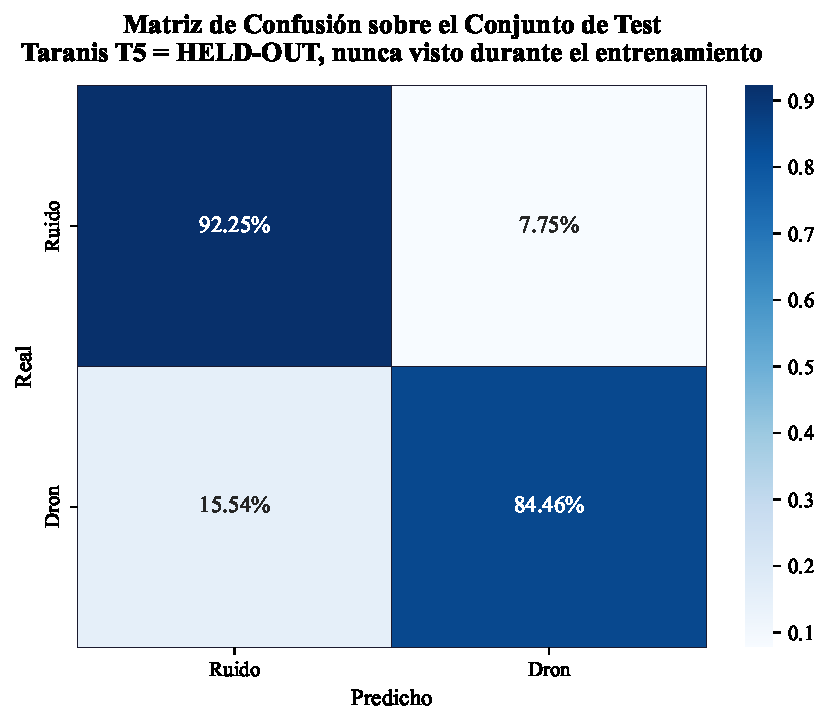
\includegraphics[width=\textwidth]{figuras/capitulo5/ht_confusion_matrix.pdf}
        \caption{Matriz de Confusión (\textit{Hard-Test}).}
        \label{fig:res_ht_cm}
    \end{subfigure}
    \hfill
    \begin{subfigure}[b]{0.56\textwidth}
        \centering
        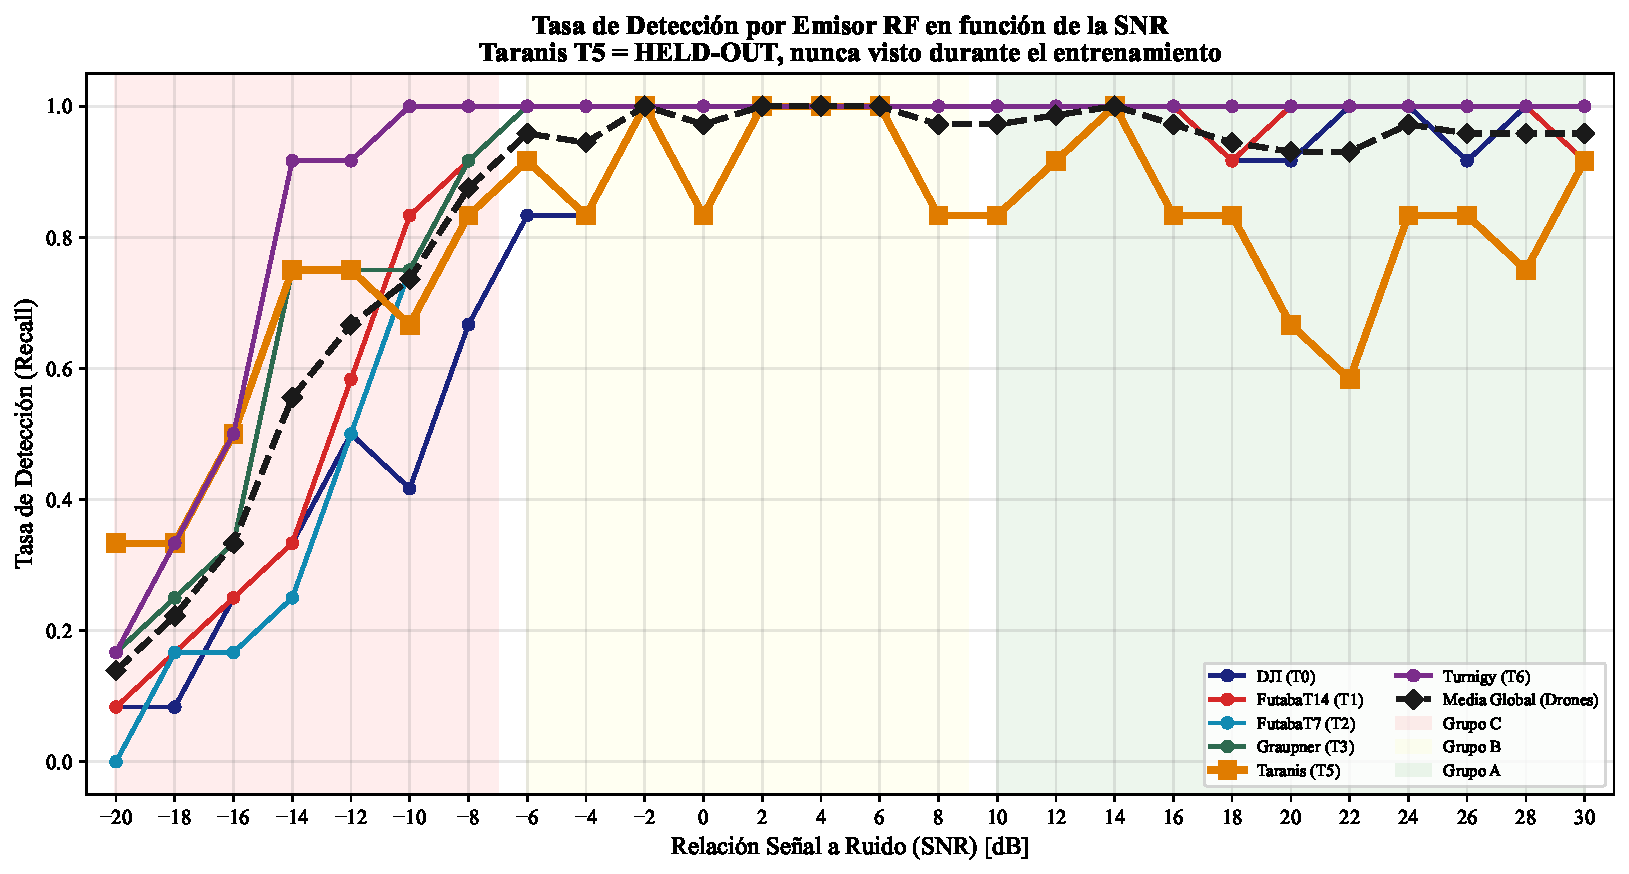
\includegraphics[width=\textwidth]{figuras/capitulo5/ht_recall_snr_lines.pdf}
        \caption{Tasa de Detección en función de la \gls{snr}.}
        \label{fig:res_ht_recall_snr}
    \end{subfigure}
    \caption{Rendimiento de generalización \textit{Zero-Shot}. El dron no visto (\textit{Target 5}) presenta una degradación predecible pero mantiene un rendimiento táctico superior al 79\%.}
    \label{fig:res_hardtest_global}
\end{figure}

Para comprender el verdadero impacto de esta exclusión, es esencial analizar no solo la métrica del emisor ausente, sino la reorganización del espacio latente completo de la red, es decir, cómo eliminar este \textit{target} del entrenamiento ha afectado al resto de predicciones del sistema. La exclusión del \textit{Target 5} implicó retirar no solo sus transmisiones activas, sino también las ventanas de ruido de fondo extraídas de sus grabaciones. Esto redujo la diversidad de la clase 0 (Ruido), lo que se tradujo en una caída de la especificidad global del modelo, que pasó del 96.74\% en la arquitectura base a un 92.25\% en la versión \textit{Zero-Shot} (Figura \ref{fig:res_ht_cm}). Como conclusión puede obtenerse que, al ver menos variabilidad de interferencias durante el entrenamiento, la red se vuelve ligeramente más propensa a la falsa alarma.

\begin{figure}[htbp]
    \centering
    \begin{subfigure}[b]{0.48\textwidth}
        \centering
        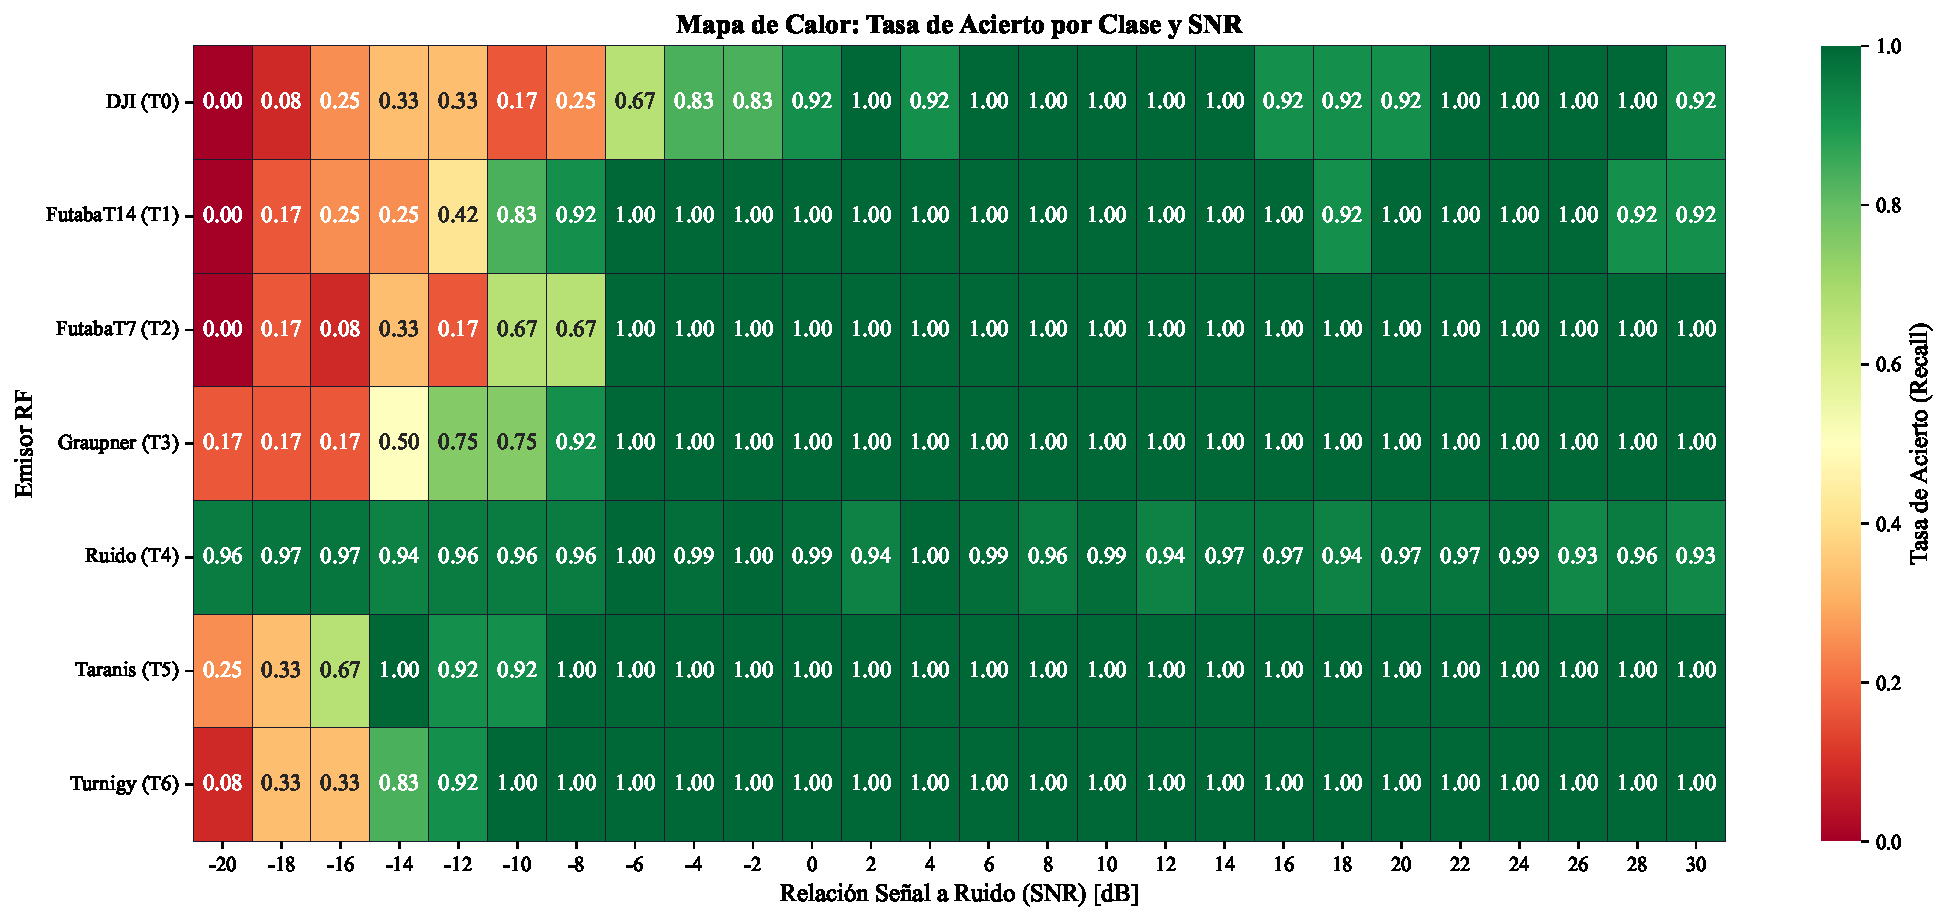
\includegraphics[width=\textwidth]{figuras/capitulo5/baseline_heatmap_snr_target.pdf}
        \caption{Modelo Base V2.1 (T5 incluido).}
        \label{fig:res_ht_heatmap_base}
    \end{subfigure}
    \hfill
    \begin{subfigure}[b]{0.48\textwidth}
        \centering
        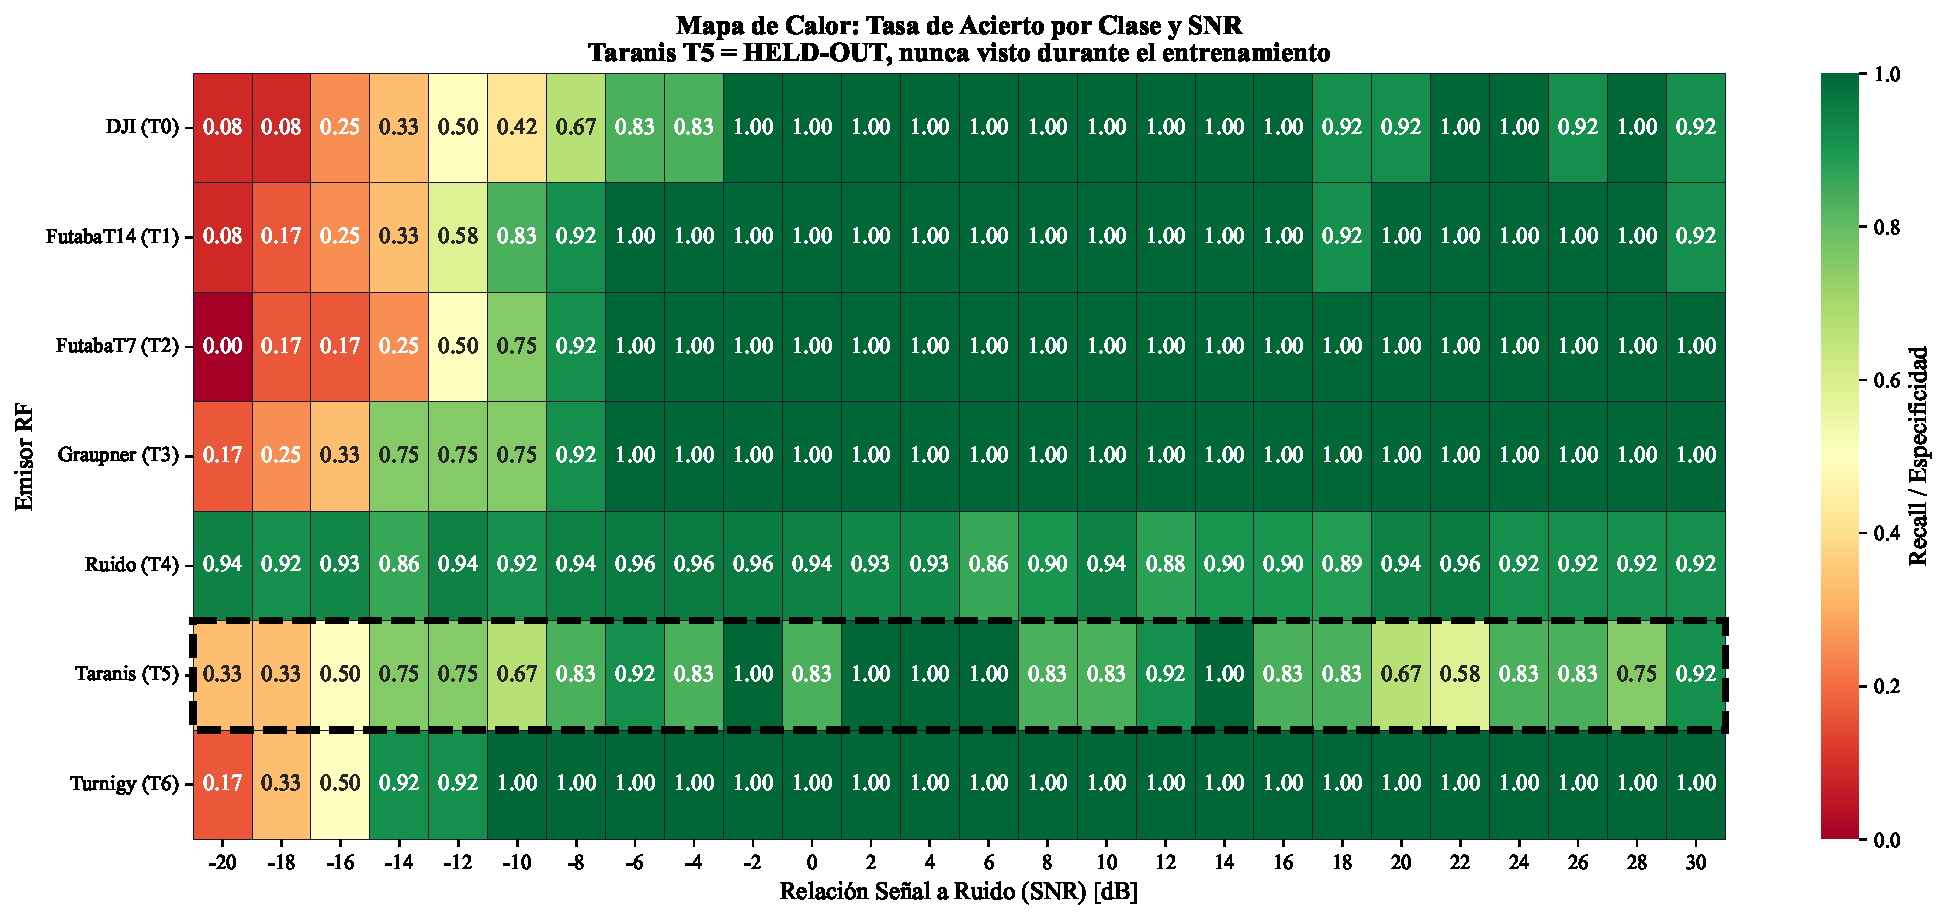
\includegraphics[width=\textwidth]{figuras/capitulo5/ht_heatmap_snr_target.pdf}
        \caption{Modelo \textit{Hard-Test} (T5 excluido).}
        \label{fig:res_ht_heatmap_ht}
    \end{subfigure}
    \caption{Comparativa de probabilidad de detección (Recall) segregada por emisor y SNR. La ceguera al \textit{Target 5} redistribuye el aprendizaje de la red hacia el resto de características canónicas FHSS.}
    \label{fig:res_hardtest_heatmaps}
\end{figure}

Analizando la capacidad de predicción sobre el resto de drones se vio que, en primer lugar, la tasa de detección (\textit{Recall}) del dron desconocido (\textit{Target 5}) evidentemente cae desde el 92.63\% (cuando formaba parte del entrenamiento) hasta el 79.17\%. Sin embargo, como ilustra la traza naranja de la Figura \ref{fig:res_ht_recall_snr}, esta degradación no es uniforme, sufriendo un colapso a niveles de relación señal a ruido extremadamente altos (SNR $> 15$ dB). A estos niveles, el canal es excepcionalmente nítido, dejando expuestas las no linealidades del oscilador y el ruido de fase microscópico exclusivos del FrSky Taranis; como el modelo nunca se ha entrenado con unas señales I/Q que sigan los patrones del emisor de este dron, la red las interpreta como una transmisión de interferencia pura no procedente de un \gls{uav}, y no se produce detección. Sorprendentemente, a niveles de SNR moderados (-5 dB a 10 dB), puede interpretarse que el ruido actúa como un regularizador: enmascara las imperfecciones únicas del \textit{hardware} desconocido y deja patente únicamente la morfología del protocolo FHSS que se comparte con el resto de dispositivos a detectar. En este régimen operativo, el modelo \textit{Hard-Test} detecta el \textit{Target 5} con mucha facilidad, validando su capacidad de abstracción y obtención de características que identifican a \gls{uav}s.

En segundo lugar, el análisis comparativo de los mapas de calor (Figura \ref{fig:res_hardtest_heatmaps}) destapa un fenómeno de \textit{transfer learning} colateral. Al suprimir la información que aporta el dron Taranis de la función de pérdida durante la fase de entrenamiento, también se suprimieron los posibles fallos de etiquetado al construir el conjunto de entrenamiento debido al ya mencionado \textit{label noise} con el que cuenta este conjunto de datos. Esto permitió a la red converger de forma mucho más pura hacia las características genéricas compartidas por el resto de drones, dando como resultado directo que el \textit{Recall} de los drones sí conocidos mejorase sistemáticamente frente al modelo base entrenado con todos los \textit{targets}: el DJI (\textit{Target 0}) mejoró un 5.45\%, el Futaba (\textit{Target 2}) un 2.56\% y el Graupner (\textit{Target 3}) un 1.92\%. 

% ==========================================
% SECCIÓN 3: DISCUSIÓN
% ==========================================
\section{Discusión}
\label{sec:discusion}

\subsection{Comparativa Estructural frente a Glüge et al. (2024)}
\label{subsec:disc_gluge}

El análisis de las arquitecturas definitivas no puede desvincularse del estado del arte sobre el que se validan. El artículo de referencia sobre el que se fundamenta este trabajo, propuesto por Glüge et al. (2024) \cite{gluge_robust_2024}, instaura una metodología fuertemente dependiente del paradigma clásico de la visión artificial aplicada al espectro electromagnético. Su diseño exige que, tras interceptar las señales I/Q, se apliquen transformadas de Fourier consecutivas para extraer espectrogramas bidimensionales. Estas imágenes alimentan posteriormente a redes convolucionales profundas de la familia VGG\footnote{Las redes VGG (\textit{Visual Geometry Group}) son una familia de arquitecturas de red neuronal convolucional muy profundas, diseñadas originalmente para la clasificación de imágenes complejas, que logran una gran precisión a costa de emplear decenas de millones de parámetros entrenables.} (concretamente desde la VGG11 hasta la VGG19). Esta aproximación bidimensional acarrea un severo incremento en el tamaño de la red: sus modelos se alojan en una escala que parte de los 9.35 millones de parámetros entrenables para su red más ligera (VGG11) y alcanza los 20.16 millones en su versión más profunda (VGG19). Esta enorme dimensionalidad aumenta drásticamente los requisitos computacionales de memoria y la demanda energética del módulo, comprometiendo su uso en campo abierto.

En contraste directo con esta premisa, la arquitectura \textit{DualStream-SlidingWindow} desarrollada en esta investigación prescinde del alto coste de procesamiento previo. Al evaluar directamente las series complejas unidimensionales junto a una estimación espectral directa, la red completa cuenta con exactamente 344.291 parámetros. Pese a esta reducción dimensional (entre 27 y 58 veces más ligera que las redes de referencia), los resultados empíricos demuestran una superioridad en el procesamiento unidimensional y una paridad frente a las técnicas de visión artificial.

Para ilustrar este hecho de forma explícita, la Figura \ref{fig:disc_gluge_comparative} presenta los resultados oficiales obtenidos en el estudio original de Glüge \textit{et al.}

\begin{figure}[htbp]
    \centering
    \begin{subfigure}[b]{0.75\textwidth}
        \centering
        
\includegraphics[width=\textwidth]{figuras/capitulo5/resultados_gluge.png}
        \caption{Resultados de Accuracy contra \gls{snr} originales del artículo de referencia (Glüge \textit{et al.}, \cite{gluge_robust_2024})}
        \label{fig:disc_gluge_original}
    \end{subfigure}
    \hfill
    \begin{subfigure}[b]{0.75\textwidth}
        \centering
        
\includegraphics[width=\textwidth]{figuras/capitulo5/DualStream-DynamicSlidingWindow/accuracy_snr_bars_local.pdf}
        \caption{Resultados de Accuracy contra \gls{snr} del modelo \textit{DualStream-DynamicSlidingWindow}}
        \label{fig:disc_gluge_overlay}
    \end{subfigure}
    \caption{Comparativa de \textit{Accuracy} frente a SNR. A la izquierda, el estado del arte comparando modelos de la familia VGG sobre espectrogramas (líneas continuas en tonos azulados con etiqueta SPEC) frente a I/Q unidimensional (líneas discontinuas en tonos ocres con etiqueta IQ). A la derecha, se muestra el rendimiento de la arquitectura CV-CNN 1D propuesta.}
    \label{fig:disc_gluge_comparative}
\end{figure}

Como se observa en la figura, sus modelos basados directamente en la señal I/Q unidimensional sufren una degradación de su rendimiento a partir de los 0 dB. Al confrontar estos resultados con los que ofrece el sistema propuesto en este trabajo, se comprueba que la red \textit{DualStream-DynamicSlidingWindow} tiene un rendimiento muy superior en todo el rango de relación señal a ruido. Concretamente, se observa que a -10 dB de \gls{snr}, las arquitecturas VGG sobre señal I/Q tienen una exactitud en torno al 70~\%; mientras que el sistema propuesto en este trabajo alcanza una \textit{accuracy} del 80~\%. En regímenes de alta \gls{snr}, el modelo propuesto también supera al de referencia, puede observarse cómo para una relación señal a ruido de 20 dB, la familia de modelos de referencia tienen una \textit{accuracy} en torno al 95~\%, mientras que el sistema implementado en este trabajo alcanza el 100~\% de exactitud. Cabe destacar que ambas soluciones presentan el mismo fenómeno a valores elevados de \gls{snr}: comienzan a perder exactitud, alcanzando su valor máximo para niveles de relación señal a ruido en torno a 5 dB y posteriormente mostrando un comportamiento descendiente. Como se ha comentado anteriormente, esto se debe a que, conforme el nivel de \gls{snr} aumenta, también aumenta la potencia de las interferencias, haciendo que los modelos tengan más dificultad para discernir entre una transmisión legítima de un dron o una interferencia. 

Además, sin requerir técnicas de visión artificial y con apenas 344 mil parámetros, la arquitectura propuesta se mantiene prácticamente a la par en niveles de exactitud con los grandes modelos bidimensionales sobre espectrogramas que proponen los autores en el artículo de referencia. Como puede observarse, la \textit{accuracy} total para niveles de potencia superiores a -2 dB en el modelo \textit{DualStream-DynamicSlidingWindow} es aproximadamente igual a la obtenida por Glüge \textit{et al.} usando la familia de modelos VGG sobre espectrogramas.

Aún más determinante resulta analizar la naturaleza de los datos evaluados. Los autores del estudio original validaron sus arquitecturas aislando y recortando vectores de señal muy cortos (16,384 muestras, equivalente a 1.2 ms), garantizando que siempre existía una ráfaga del dron en los datos de entrada en la fase de entrenamiento. Esta estrategia eliminaba el problema estadístico más grave con el que se ha tenido que lidiar en esta investigación: el ruido de etiquetas o \textit{label noise}. En contrapartida, el sistema propuesto en este trabajo se ha visto obligado a inferir directamente sobre grabaciones completas de 75 ms, asumiendo la responsabilidad de detectar los escasos períodos activos del dron e ignorar los silencios dominados por el ruido del canal o las interferencias.

% CORREGIDA: contradicción técnica sobre Edge AI.
% La arquitectura NO está "diseñada nativamente" para Edge AI en el alcance actual del TFM.
% Se argumenta la viabilidad futura basándose en la reducción de parámetros.
La relevancia de haber logrado esta robustez predictiva bajo condiciones más adversas reside en su traslación tecnológica potencial. Reducir los pesos de la red a 344 mil parámetros elimina el cuello de botella computacional del enfoque en 2D. Esta reducción paramétrica hace que la arquitectura 1D resulte viable para su posterior despliegue sobre plataformas de radio definida por software (SDR) de bajo coste o procesadores embebidos. Si bien el alcance del presente trabajo no comprende la optimización final del modelo para la inferencia en tiempo real en hardware de borde (\textit{Edge AI}), la dimensionalidad conseguida constituye el primer paso técnico necesario hacia ese escenario, a diferencia de las redes VGG analizadas, cuyas decenas de millones de parámetros las excluyen de facto de ese ámbito.

\subsection{Análisis de Latencia e Inferencia Computacional}
\label{subsec:latencia_inferencia}

La viabilidad operativa de una arquitectura orientada a su despliegue en nodos de \textit{Edge AI} no puede evaluarse exclusivamente en base a su tasa de acierto o F1-Score; el coste computacional y la latencia de inferencia constituyen factores limitantes críticos para el procesamiento en tiempo real de ráfagas continuas. Con el objetivo de cuantificar este impacto, se ha llevado a cabo un análisis empírico de latencia sobre las tres iteraciones arquitectónicas principales desarrolladas a lo largo de este Trabajo Fin de Máster.

Las pruebas se han ejecutado de manera local utilizando una unidad de procesamiento gráfico (GPU) estandarizada (arquitectura CUDA), procesando de manera secuencial tensores correspondientes a ráfagas de 75\,ms de duración. Para garantizar la validez estadística y evitar el sobrecoste derivado de la inicialización de los grafos computacionales dinámicos en memoria, se realizaron 50 iteraciones previas de calentamiento (\textit{warm-up}) seguidas de 1.000 iteraciones cronometradas en régimen estacionario, midiendo el tiempo de ejecución estricto de la pasada hacia adelante (\textit{forward pass}). Los resultados consolidados en milisegundos se muestran en la Tabla \ref{tab:latency_benchmark}.

\begin{table}[htbp]
\centering
\caption{Comparativa empírica de latencia de inferencia por ráfaga (75\,ms)}
\label{tab:latency_benchmark}
\begin{tabular}{l c c c}
\toprule
\textbf{Arquitectura} & \textbf{Dominios de Entrada} & \textbf{Flujo Operativo} & \textbf{Latencia Media (ms)} \\
\midrule
SingleStream CV-CNN & I/Q & Ráfaga completa (1 iteración) & 7,71 $\pm$ 0,57 \\
DualStream (V2.1) & I/Q + PSD & Ráfaga completa (1 iteración) & 1,40 $\pm$ 0,33 \\
DualStream (V2.2) & I/Q + PSD & Ventana deslizante (16 iteraciones) & 41,89 $\pm$ 8,47 \\
\bottomrule
\end{tabular}
\end{table}

Estos resultados demuestran de forma empírica la alta eficiencia del diseño. Sorprendentemente, el modelo dual resulta ser más rápido (1,40 ms) que la arquitectura base \textit{SingleStream} (7,71 ms). Este fenómeno se explica matemáticamente por las dimensiones de los mapas de características: la red base emplea extracciones de \textit{features} excesivamente grandes en sus primeras capas para compensar la falta de información en el dominio de frecuencia, aumentando el número de operaciones de multiplicación realizadas. Al aportar directamente la \gls{psd} precalculada, la arquitectura bimodal realiza la inferencia de forma mucho más rápida usando las \textit{features} que se extraen de esta rama.

Finalmente, la implementación operativa definitiva mediante ventana deslizante con mitigación adaptativa de ruido (\textit{DualStream-SlidingWindow}), que requiere ejecutar el modelo de forma iterativa 16 veces por cada ráfaga de 75\,ms para blindar la especificidad de la detección, arroja una latencia acumulada de apenas 41,89 milisegundos. Dado que este tiempo de cómputo es inferior a la duración de la grabación de entrada (75\,ms), el sistema es matemáticamente capaz de procesar la ventana de captura completa antes de que se tenga otra lista para ser analizada. Este hito confirma que la arquitectura final sería plenamente viable como sensor de vigilancia pasiva en tiempo real.

\subsection{Análisis Global del Estado del Arte}
\label{subsec:disc_sota}

Para contextualizar de manera exhaustiva el alcance de la arquitectura de evaluación continua propuesta, la Tabla \ref{tab:sota_comparative} expone una matriz técnica enfrentando las propiedades del diseño frente a los repositorios de datos y algoritmos imperantes documentados en la literatura académica reciente.

\begin{table}[H]
\centering
\resizebox{\textwidth}{!}{
\begin{tabular}{l c c c c c}
\toprule
\textbf{Métrica / Capacidad} & \textbf{\cite{allahham_dronerf_2019}} & \textbf{\cite{zhao_drone_2024}} & \textbf{\cite{zheng_multi-scenario_2026}} & \textbf{\cite{gluge_robust_2024}} & \textbf{Este Trabajo} \\
\midrule
Conjunto de datos evaluado & DroneRF & UAVSig & DRFF-R2 & NoisyUAV v2 & NoisyUAV v2 \\
Ruido interferente (Wi-Fi/BT) & No & No & Sí & Sí & \textbf{Sí} \\
Evaluación en SNR extrema ($<0$ dB) & No & No & No & Sí & \textbf{Sí} \\
Inclusión de clase exclusiva de ruido & No & Sí & Sí & Sí & \textbf{Sí} \\
Inferencia sin pre-segmentación & No & No & No & No & \textbf{Sí} \\
Mitigación adaptativa de ruido (CFAR) & No & No & No & No & \textbf{Sí} \\
Dominio de entrada principal & I/Q & PSD / 2D & I/Q & PSD / 2D & \textbf{I/Q y PSD} \\
Conservación de la fase compleja & Sí & No & Sí & No & \textbf{Sí} \\
Algoritmo de clasificación & SVM / RF & CNN 2D & ViT / LLM & CNN 2D & \textbf{CV-CNN 1D} \\
Tamaño del modelo (Parámetros) & Bajo & Alto & Alto & Muy alto ($>9$M) & \textbf{Bajo (344k)} \\
Viabilidad para \textit{Edge AI} & Sí & No & No & No & \textbf{Sí} \\
\bottomrule
\end{tabular}
}
\caption{Matriz comparativa de capacidades y restricciones entre la literatura contemporánea y el sistema propuesto.}
\label{tab:sota_comparative}
\end{table}

La tabla refleja que el enfoque mayoritario en la comunidad científica centra sus validaciones sobre capturas limpias pre-segmentadas o bajo regímenes limitados por una buena relación señal a ruido. Las arquitecturas que sí abordan el problema bajo saturación (\cite{gluge_robust_2024}) asumen el sacrificio computacional de desechar la matriz temporal compleja I/Q en favor del tratamiento 2D clásico, descartando la información de fase y reduciendo su viabilidad para la inferencia móvil. El modelo propuesto en este trabajo ofrece una solución de compromiso donde se garantizan las exigencias críticas de detección requeridas por la defensa perimetral sin sobrepasar la capacidad de cómputo de procesadores embebidos de bajo consumo.